\documentclass{beamer}

\mode<presentation> {
}

\usepackage{graphicx} % Allows including images
\usepackage{booktabs} % Allows the use of \toprule, 
\usepackage{longtable} % Allows the use of \toprule, 



\title[]{Bayesian Clinical Trials} 
\subtitle{An introduction to the Beta-Binomial model} 
\date{} 


\begin{document}

\begin{frame}
\titlepage % Print the title page as the first slide
\end{frame}


\begin{frame}{Background}

For a phase IIA trial, suppose our goal is to evaluate the response rate
\(\pi\) for a new drug by testing the hypotheses
\[H_{0}: \pi \le p_{0} \phantom{0}H_{1}: \pi \ge p_{1}\]

Suppose we set a maximum number of accrued patients \(N_{max}\), and
assume that the number of responses \(X\) among the current \(n\)
patients follows a Binomial distribution with parameter \(\pi\). The
binomial likelihood is:
\[f\left(x|\pi,n\right)=\binom{n}{x} \pi^{x}\left(1-\pi\right)^{1-x}\]

\end{frame}

\begin{frame}{Prior}

We assume that the prior distribution of the response rate, \(\pi\),
follows a Beta distribution:
\[g\left(\pi\right)=Beta\left(c,d\right)=B\left(c,d\right)^{-1}\pi^{c-1}\left(1-\pi\right)^{d-1}\]

The quantity \(c/\left(c + d\right)\) gives the prior mean, while the
magnitude of \(c + d\) indicates how informative the prior is. The
larger this sum, the more informative the prior and the stronger the
belief it contains.

\end{frame}

\begin{frame}{The conjugacy property}

By the conjugacy of the beta prior and binomial likelihood, the
posterior distribution of the response rate follows a beta distribution
with parameters \(c+x\) and \(d+n-x\):
\[f\left(\pi|x,n,c,d\right)=\frac{f\left(x|\pi,n\right)g\left(\pi\right)}{\int_0^1 f\left(x|\pi,n\right)g\left(\pi\right) d\pi}\]
\[f\left(\pi|x,n,c,d\right)= \frac {\pi^{c+x-1}\left(1-\pi\right)^{d+n-x-1}} {B\left(c+x,d+n-x\right)}\]

Whenever we have a prior that is conjugate to the likelihood, the
posterior distribution belongs to the same family of distributions as
the prior. As a consequence, conjugate priors are extremely useful tools
in Bayesian statistics, since they make things a lot more analytically
tractable.

\end{frame}

\begin{frame}{Posterior distribution}

Once we have computed (or obtained an estimate of) the posterior,
inference comes down merely to summarizing this distribution, since by
Bayes' Rule the posterior summarizes everything we know about the model
parameters in light of the data.

\end{frame}

\begin{frame}{Example}

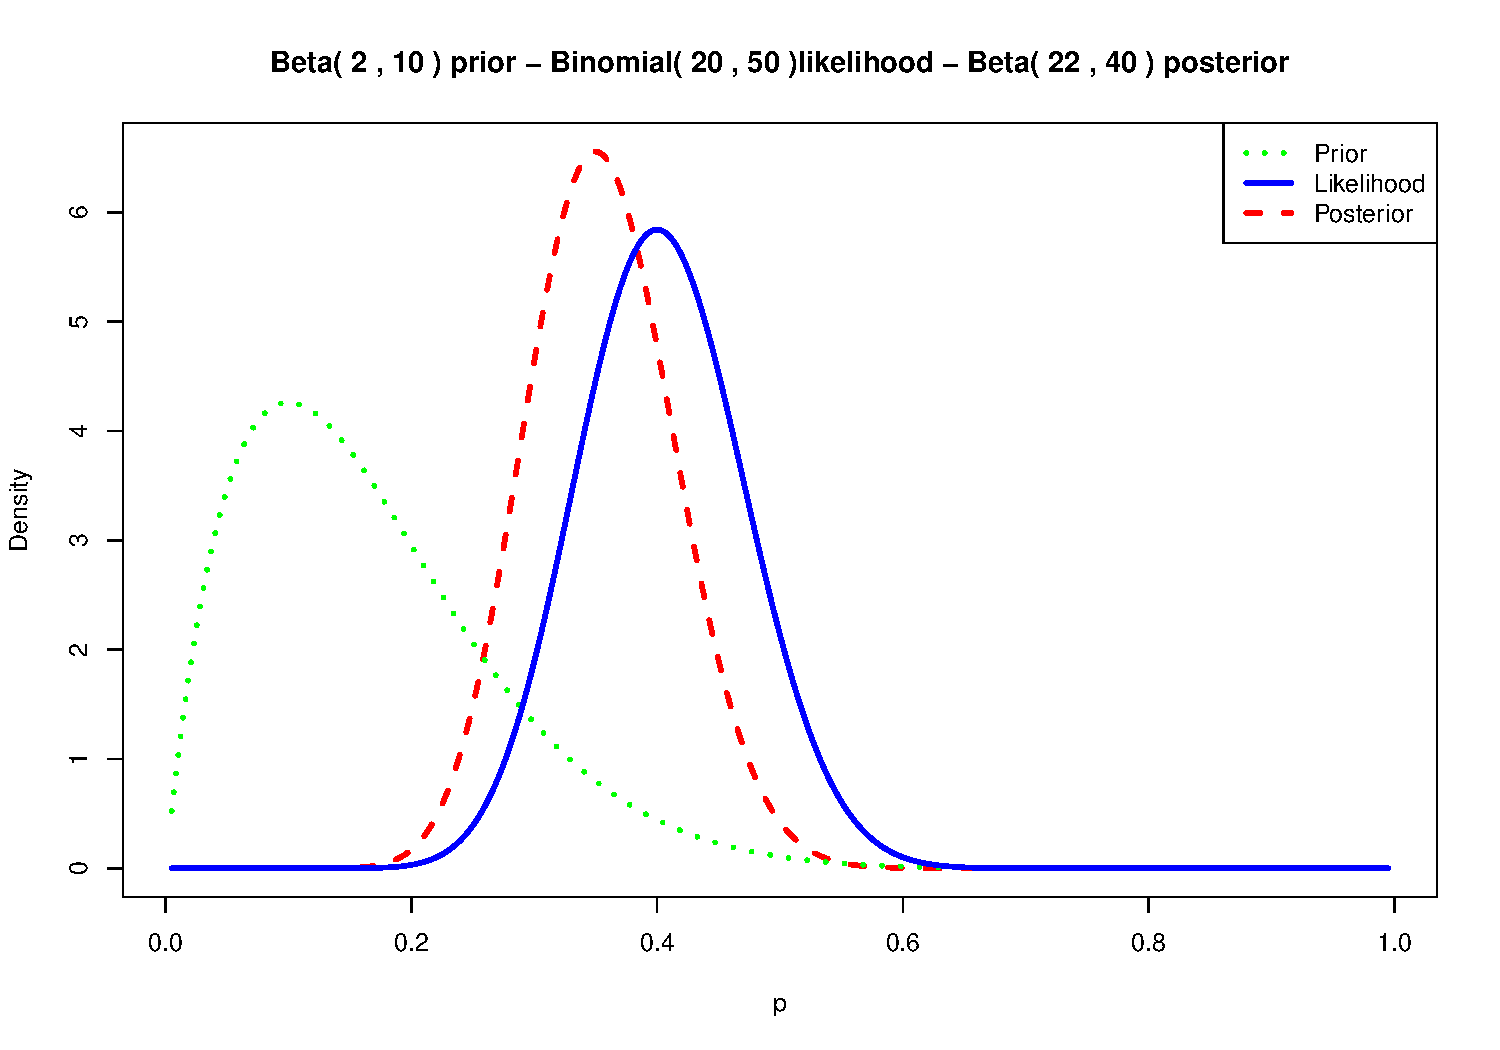
\includegraphics[scale=0.4]{04BetaBinomialModel_files/figure-beamer/unnamed-chunk-1-1.pdf}

\end{frame}

\begin{frame}{Posterior predictive probability}

Suppose that you've constructed a beta-binomial model for data on the
current \(n\) patients and you want to make a prediction about what you
expect to happen next. The first thing that we might want to know is the
posterior mean; that is, our best point estimate for \(\pi\). This is
given by:

\[
E\left(\pi|x,n,c,d\right)=\int_0^1 {\pi f\left(\pi|x,n\right) d\pi}=...=\left(c+x\right)/\left(c+d+n\right)
\]

What about the more general prediction about future data?

\end{frame}

\begin{frame}

Imagine that we then aim to enroll an additional \(m\) patients. What is
the probability that exactly \(i\) of these are successes?

\[
f\left(i|m,n,x,c,d\right)=\int_0^1 {f\left(i|\pi,m\right)f\left(\pi|n,x,c,d\right) d\pi}
\]

The general name for the expected distribution over future observations
is the posterior predictive distribution. If the prior distribution is
\(Beta\left(c,d\right)\) and the likelihood is
\(Binomial\left(n,\pi\right)\), then the posterior predictive
distribution is a \(Beta-Binomial\left(m,c+x,d+n-x\right)\)
distribution.

\end{frame}

\begin{frame}

The predictive probability approach looks into the future based on the
current observed data to project whether a positive conclusion at the
end of study is likely or not, and then makes a sensible decision at the
present time accordingly.

Suppose that we can claim for efficacy is the posterior probability of
\(\pi\) exceeding \(p_{0}\) is greater than a threshold value
\(\gamma\). Let Y be the number of responses of \(m\) future patients
following a \(Beta-Binomial\left(m,c+x,d+n-x\right)\) distribution.\\We
can calculate the predictive probability (PP) of trial success as: \[
PP=\sum_{i=0}^{m}{P\left(Y=i\right|x)}\phantom{0} I\left[P\left(\pi>p_{0}|x,Y=i\right)>\gamma\right]
\]

\end{frame}

\begin{frame}

A high PP means that the treatment is likely to be efficacious by the
end of the study, given the current data, whereas a low PP suggests that
the treatment may not have suffcient activity. We define a rule by
introducing two thresholds on PP:

\begin{itemize}
\itemsep1pt\parskip0pt\parsep0pt
\item
  if \(PP<\gamma_{lower}\) then stop the trial and reject \(H_{1}\)
\item
  if \(PP>\gamma_{upper}\) then stop the trial and reject \(H_{0}\)
\item
  otherwise continue accrual till reaching \(N_{max}\)
\end{itemize}

For phase IIA trials, we often prefer to choose \(\gamma_{lower}>0\) and
\(\gamma_{upper}=1\) to allow early stopping due to futility, but not
due to efficacy.

\end{frame}

\begin{frame}{References}

\begin{itemize}
\itemsep1pt\parskip0pt\parsep0pt
\item
  Berry S.M., Carlin B.P., Lee J.J. , Muller P. Bayesian Adaptive
  Methods for Clinical Trials. 2011 Chapman \& Hall.
\end{itemize}

\end{frame}


\end{document}